\chapter{System Architecture}     
        The system architecture organizes the system's necessities into manageable blocks as shown in figure \ref{fig:systemstructure}.
        It is essentially divided into two major components, the Social Routing Client Application \cite{clientapplicationdocs} and the Social Routing Service with a third one being the external services.
        
        \vfill
        \begin{figure}[h]            
            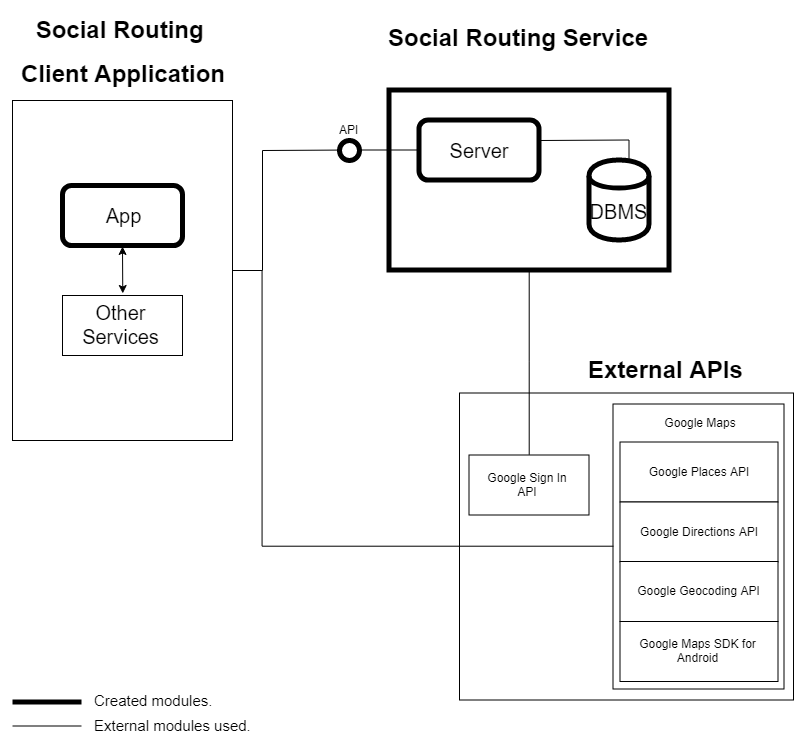
\includegraphics[width=\textwidth]{images/project-structure/system-structure.PNG}
            \caption{System structure.}
            \label{fig:systemstructure}
        \end{figure}  

        The Social Routing Service is subdivided into two components, the Server and the Database Management System. The Server exposes its
        functionality through an HTTP\cite{httponlinedocs} API\cite{api} (Social Routing API \cite{apidocs}) and as such, receives requests from a client, processes the received request and responds accordingly.
        The Database Management System is used to store the server's data, over which the necessary calculations are made.\par The Social 
        Routing Service uses only one external API, Google Sign In\cite{googlesignindocs}, which is used to help with user authentication. Although the Social Routing
        service was built along the Client side application, any HTTP client that follows the service's API documentation is able to make requests
        to it.        

        The role of the Social Routing Client Application is to provide an interface to Android \cite{androiddocs} devices which the user can interact with, to expose the project 
        idea and essentially to demonstrate the Social Routing Service functionalities to the client. This component communicates with the Social Routing Service and 
        external services when required, through the HTTP protocol. The external services are APIs provided by the Google Maps platform \cite{googlemapsplatform} 
        to retrieve information such as the user profile from google accounts and content that helps managing the the Google maps, like locations, places and routes. This component
        also communicates with Internal Services which are used to facilitate the client side development and to materialize communication with the external services.